\subsubsubsubsection{StreetBuilder}
\begin{figure}[h]
\centering
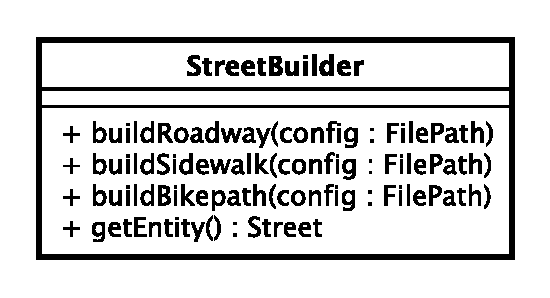
\includegraphics[scale=0.6,keepaspectratio]{images/solution/street_builder.eps}
\caption{\pReactiveBuild::StreetBuilder}
\label{fig:sd-app-street_builder}
\end{figure}
\FloatBarrier
\begin{itemize}
  \item \textbf{\descr} \\
    It represents the builder of street entities. 
  \item \textbf{\ops}
  \begin{itemize} 
    \item[+] \texttt{buildRoadway(config: FilePath)} \\
Builds a roadway using roadwayfactory according to a specific configuration.
    \item[+] \texttt{buildSidewalk(config: FilePath)} \\
Builds a sidewalk using sidewalkfactory according to a specific configuration.
    \item[+] \texttt{buildBikepath(config: FilePath)} \\
Builds a bikepath using bikepathfactory according to a specific configuration.
    \item[+] \texttt{getEntity() : Street} \\
Returns the street.
  \end{itemize}
\end{itemize}
